\chapter{Conclusions and project plan}

The plan of work is to first use a basic model, part of speech tagging, Wordnet and regular expressions to extract potential training data from some text source e.g. English Wikipedia. These examples will then be hand labelled to start building a training data set. They will be used to create a more sophisticated model that at first will use the features laid out in Speech and Language Processing by \cite{reference1} shown here.

\begin{figure}[hbt!]
\centering
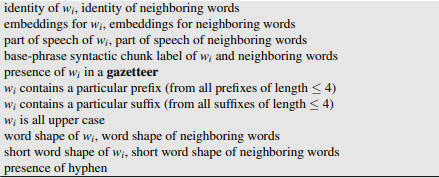
\includegraphics[width=0.75\textwidth]{figures/features.png}
\caption{Features to train the NER model}
\end{figure}

A feedback tool will be implemented here for to more efficiently train the model. This tool will allow me to label found tokens are either correct or incorrect. If the token was misidentified, then the tool will also allow me to correct it. This will give a base level from which the rest of the project can be built upon. Reaching this stage will be critical as the feasibility of the project can start being assessed more closely. Additional investigation and research may be required if the model isn’t performing as expected.

Additionally, more investigation will be done into proper techniques for relationship extraction as well as building a database model for storing the collected results. From here we can start to think about other ways to increase the model’s accuracy by checking for previous records of objects and possibly estimating size based on object hierarchy.

These stages for the most part can all happen simultaneously, other than needing training data to build the second set of models, the stages will progress alongside one another. This is shown in figure 5.2.

\begin{figure}[hbt!]
\centering
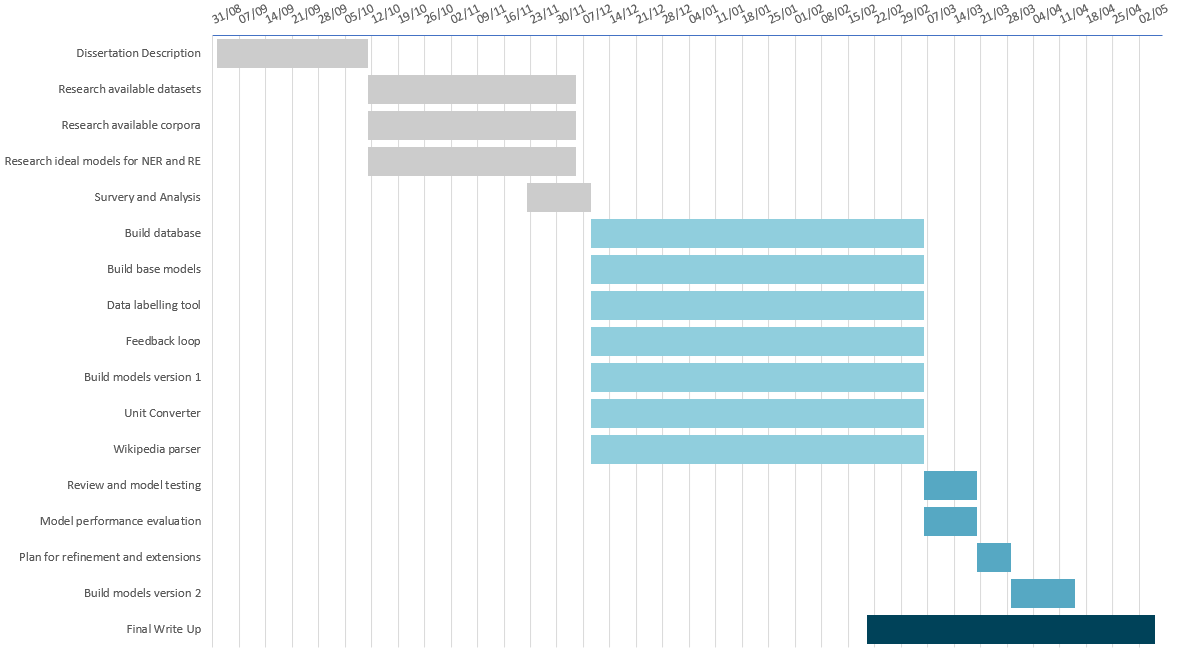
\includegraphics[width=0.75\paperwidth]{figures/gantt.png}
\caption{Project timeline}
\end{figure}